\documentclass{article}

\def\ParSkip{} 
% Packages
\usepackage{amssymb,amsmath,amsthm,bbm}
\usepackage{verbatim,float,url,dsfont}
\usepackage{graphicx,subfigure,psfrag}
\usepackage{algorithm,algorithmic}
\usepackage{mathtools,enumitem}
\usepackage{multirow}
\usepackage{ragged2e}
\usepackage{xr-hyper}
\usepackage{array}

\usepackage[colorlinks=true,citecolor=blue,urlcolor=blue,linkcolor=blue]{hyperref}
\usepackage[margin=1in]{geometry}
\usepackage[round]{natbib}

\usepackage[utf8]{inputenc} % allow utf-8 input
\usepackage[T1]{fontenc}    % use 8-bit T1 fonts
\usepackage{booktabs}       % professional-quality tables
\usepackage{nicefrac}         % compact symbols for 1/2, etc.
\usepackage{microtype}      % microtypography

\ifdefined\TimesFont 
\usepackage{times} % use times font
\fi

\ifdefined\ParSkip 
\usepackage{parskip} % use par skip
\fi

% Theorems and such
\newtheorem{theorem}{Theorem}
\newtheorem{lemma}{Lemma}
\newtheorem{corollary}{Corollary}
\newtheorem{proposition}{Proposition}
\theoremstyle{definition}
\newtheorem{remark}{Remark}
\newtheorem{definition}{Definition}

% Assumption
\newtheorem*{assumption*}{\assumptionnumber}
\providecommand{\assumptionnumber}{}
\makeatletter
\newenvironment{assumption}[2]{
  \renewcommand{\assumptionnumber}{Assumption #1#2}
  \begin{assumption*}
  \protected@edef\@currentlabel{#1#2}}
{\end{assumption*}}
\makeatother

% Widebar
\makeatletter
\newcommand*\rel@kern[1]{\kern#1\dimexpr\macc@kerna}
\newcommand*\widebar[1]{%
  \begingroup
  \def\mathaccent##1##2{%
    \rel@kern{0.8}%
    \overline{\rel@kern{-0.8}\macc@nucleus\rel@kern{0.2}}%
    \rel@kern{-0.2}%
  }%
  \macc@depth\@ne
  \let\math@bgroup\@empty \let\math@egroup\macc@set@skewchar
  \mathsurround\z@ \frozen@everymath{\mathgroup\macc@group\relax}%
  \macc@set@skewchar\relax
  \let\mathaccentV\macc@nested@a
  \macc@nested@a\relax111{#1}%
  \endgroup
}
\makeatother

% Min and max
\newcommand{\argmin}{\mathop{\mathrm{argmin}}}
\newcommand{\argmax}{\mathop{\mathrm{argmax}}}
\newcommand{\minimize}{\mathop{\mathrm{minimize}}}
\newcommand{\maximize}{\mathop{\mathrm{maximize}}}
\newcommand{\st}{\mathop{\mathrm{subject\,\,to}}}

% Shortcuts
\def\R{\mathbb{R}}
\def\C{\mathbb{C}}
\def\Z{\mathbb{Z}}
\def\N{\mathbb{N}}
\def\E{\mathbb{E}}
\def\P{\mathbb{P}}
\def\T{\mathsf{T}}
\def\Cov{\mathrm{Cov}}
\def\Var{\mathrm{Var}}
\def\indep{\perp\!\!\!\perp}
\def\th{^{\text{th}}}
\def\tr{\mathrm{tr}}
\def\df{\mathrm{df}}
\def\dim{\mathrm{dim}}
\def\col{\mathrm{col}}
\def\row{\mathrm{row}}
\def\nul{\mathrm{null}}
\def\rank{\mathrm{rank}}
\def\nuli{\mathrm{nullity}}
\def\spa{\mathrm{span}}
\def\sign{\mathrm{sign}}
\def\supp{\mathrm{supp}}
\def\diag{\mathrm{diag}}
\def\aff{\mathrm{aff}}
\def\conv{\mathrm{conv}}
\def\dom{\mathrm{dom}}
\def\hy{\hat{y}}
\def\hf{\hat{f}}
\def\hmu{\hat{\mu}}
\def\halpha{\hat{\alpha}}
\def\hbeta{\hat{\beta}}
\def\htheta{\hat{\theta}}
\def\cA{\mathcal{A}}
\def\cB{\mathcal{B}}
\def\cD{\mathcal{D}}
\def\cE{\mathcal{E}}
\def\cF{\mathcal{F}}
\def\cG{\mathcal{G}}
\def\cK{\mathcal{K}}
\def\cH{\mathcal{H}}
\def\cI{\mathcal{I}}
\def\cL{\mathcal{L}}
\def\cM{\mathcal{M}}
\def\cN{\mathcal{N}}
\def\cP{\mathcal{P}}
\def\cS{\mathcal{S}}
\def\cT{\mathcal{T}}
\def\cW{\mathcal{W}}
\def\cX{\mathcal{X}}
\def\cY{\mathcal{Y}}
\def\cZ{\mathcal{Z}}


\title{Nonparametric Regression: Nearest Neighbors and Kernels \\ \smallskip 
\large Advanced Topics in Statistical Learning, Spring 2023 \\ \smallskip
Ryan Tibshirani}
\author{}
\date{}

\begin{document}
\maketitle
\RaggedRight
\vspace{-50pt}

\section{Introduction}

Given a random pair $(X,Y) \in \R^d \times \R$, recall that the function 
\[
 f_0(x) = \E(Y|X=x) 
\]
is called the regression function (of $Y$ on $X$).  The basic goal in
nonparametric regression is to construct an estimate \smash{$\hf$} of $f_0$ 
without assuming a specific parametric form for $f_0$, and instead only assuming 
that $f_0$ is smooth in some way.

We typically estimate \smash{$\hf$} from i.i.d.\ samples $(x_i,y_i) \in \R^d
\times \R$, $i=1,\dots,n$ that have the same joint distribution as $(X,Y)$. We 
often call $X$ the \emph{input}, \emph{predictor}, \emph{feature}, etc., and $Y$
the \emph{output}, \emph{outcome}, \emph{response}, etc. Remember that we called
this the XY-Pairs model, which is equivalent to the Random-X signal plus noise
model:  
\begin{gather*}
y_i = f_0(x_i) + \epsilon_i, \; \text{where $\E[\epsilon_i] = 0$}, \\
\text{$\epsilon_i$, $i=1,\dots,n$ are i.i.d.}, \\
\text{and $x_i$, $i=1,\dots,n$ are i.i.d.}  
\end{gather*} 
If we \emph{additionally assume that each $x_i \indep \epsilon$}, then recall we 
can condition on $x_i$, $i=1,\dots,n$, and we get the Fixed-X signal plus noise
model:  
\begin{gather*}
y_i = f_0(x_i) + \delta_i, \; \text{where $\E[\delta_i] = 0$}, \\
\text{$\delta_i$, $i=1,\dots,n$ are i.i.d.}, \\  
\text{and $x_i$, $i=1,\dots,n$ are fixed.}   
\end{gather*}

For the theory we will present in what follows, we will assume that each $x_i
\indep \epsilon$ (recall from the review lecture that this is not a completely
innocuous assumption). Hence we will take the liberty of viewing $x_i$,
$i=1,\dots,n$ as random or fixed---simply adopting whichever perspective is
convenient at any given point. For example, we may treat them as fixed in some
key parts of an analysis, and then integrate over them at the end.    

This is done for simplicity and we should note that most of the classic theory
in nonparametric regression can be done without the assumption that $x_i \indep
\epsilon$; e.g., see \citet{gyorfi2002distribution} (however, in exchange for
removing this assumption, they typically make an assumption about boundedness of 
the features).     

\subsection{Notation}

For nonrandom sequences $a_n,b_n$, we will write $a_n \lesssim b_n$ to mean $a_n
= O(b_n)$, and for a random sequence $A_n$, we say ``$A_n \lesssim b_n$ in
probability'' to mean $A_n = O_p(b_n)$. This just simplifies our notation a bit
when $b_n$ is a power of $n$ with a fractional exponent. We also use $a_n \asymp 
b_n$ to mean $a_n = O(b_n)$ and $b = O(a_n)$. 

Given $x_1\dots,x_n$, recall that the $L^2(P_n)$ norm, where $P_n$ is the
empirical distribution of $x_1\dots,x_n$, is defined by 
\[
\|f\|_n^2 = \frac{1}{n} \sum_{i=1}^n f^2(x_i).
\]
You'll often see this written as \smash{$\|\cdot\|_{L^2(P_n)}$}, but in this
document we'll abbreviate this by $\|\cdot\|_n$, and we'll call this the 
\emph{empirical norm}.

For $x_0 \sim P$, recall that the $L^2(P)$ norm is defined by 
\[
\|f\|_2^2 = \E[f^2(x_0)] = \int f^2(x) \, dP(x). 
\]
Again, you'll often see this written as \smash{$\|\cdot\|_{L^2(P)}$}, but in
we'll abbreviate this by $\|\cdot\|_2$, and we'll call this the \emph{population
  norm}.    

Key quantities of interests will be the in-sample and out-of-sample error
incurred by an estimator \smash{$\hf$} of $f_0$, which are, respectively, 
\[
\|\hf - f_0\|_n^2 \quad \text{and} \quad \|\hf - f_0\|_2^2.
\]
In either case, this is a random quantity (since \smash{$\hf$} is itself
random). We will study bounds in probability or in expectation,\footnote{In the 
  review lecture, we were more precise about using ``error'' and ``risk'' to
  mean separate things; and defined the risk via the expectations 
  \smash{$\E\|\hf - f_0\|_n^2$} and \smash{$\E\|\hf - f_0\|_2^2$}, with respect  
  to appropriate randomness in the training set that is used to define
  \smash{$\hf$}. In this lecture, we'll take the liberty of being more flexible
  with our nomenclature.}     
depending on what is more convenient in the given analysis. In this vein, when
we write 
\[
\E\|\hf - f_0\|_n^2 \lesssim b_n \quad \text{or} \quad \E\|\hf - f_0\|_2^2
\lesssim b_n \quad \text{in probability},
\]
the expectations are to be generally interpreted as being over all that is
random \emph{except} for the inputs $x_i$, $i=1,\dots,n$, whose distribution
governs the ``in probability'' statement. When we write expectation bounds
without the ``in probability'' qualifier, the expectations are over all that is
random.

\subsection{What does ``nonparametric'' mean?}

Importantly, in nonparametric regression we don't assume a particular parametric
model for $f_0$. Still, in many approaches, we estimate $f_0$ using a linear
combination of basis functions, written as   
\[
\hf(x) = \sum_{j=1}^m \hbeta_j g_j(x). 
\]
A common question that comes to mind when learning this material: aren't the
coefficients on the basis functions parameters? And so ... how is this
nonparametric?      

To be clear, the point is that \emph{we don't assume a parametric form for
  $f_0$}, i.e., we don't assume $f_0$ is itself a linear combination of
$g_1,\dots,g_m$. In this sense, the estimated coefficients
\smash{$\hbeta_1,\dots,\hbeta_m$} are not really viewed as parameter estimates; 
and we are not concerned with how close they are to some ``true'' parameters. We 
only care about how close \smash{$\hf$} is to $f_0$.

Of course, in order for this to ``work'', we need our representation to be
sufficiently flexible---otherwise we can't guarantee \smash{$\hf$} will be close 
$f_0$. The gap between our representation and $f_0$ is known as the
\emph{approximation error}. Sometimes this will be an explicit part of the
analysis (e.g., with splines) and sometimes it won't (e.g., with kernels). Here
is a concrete example: for any $f_0 : [0,1] \to \R$ whose second derivative is
integrable, and any points $t_1,\dots,t_N \in [0,1]$, there exists a cubic
spline \smash{$\bar{f}$} with knots at $t_1,\dots,t_N$ (to be defined precisely
in the splines lecture) such that
\[
\|\bar{f} - f_0\|_\infty \leq \frac{c}{N} \bigg[ \int_0^1 [f_0''(x)]^2 \, dx
\bigg]^{1/2},  
\]
where $c>0$ is a constant and $\|f\|_\infty = \sup_{x \in [0,1]} \, |f(x)|$ is
the $L^\infty$ norm on $[0,1]$. Note that \smash{$\int_0^1 [f_0''(x)]^2 \, dx$}
is a measure of the smoothness of $f_0$. If this remains constant, and we choose 
\smash{$N=\sqrt{n}$}, then the squared $L^2$ approximation error---either in 
empirical or population norm (\smash{$\|\bar{f} - f_0\|_n^2$} or
\smash{$\|\bar{f} - f_0\|_2^2$})---will be on the order of $1/n$, which will be  
negligible relative to the overall estimation error that we will encounter.

\subsection{What we cover here}

The goal is to expose you to a variety of methods over the next several lectures
on nonparametric regression, and give you a flavor of some interesting results,
under different assumptions.  A few topics we will cover into more depth than
others, but overall, this will be far from a complete treatement of
nonparametric regression (that would take a whole course, or more).  

Of the many texts you can consult for more details, proofs, etc., we highlight
\citet{gyorfi2002distribution, wasserman2006all, tsybakov2009introduction} as
general references on theory; \citet{hastie2009elements} as a general reference
on methods; and \citet{vandegeer2000empirical, wainwright2019high} for analysis
techniques and probabilistic tools.

Throughout, our discussion will bounce back and forth between the univariate
case ($d=1$) and multivariate case ($d>1$). Some methods have obvious (natural) 
multivariate extensions; some don't. Nevertheless, we can always use
low-dimensional (even just univariate) nonparametric regression methods as
building blocks for a high-dimensional nonparametric estimator.  We'll study
this later, when we talk about additive models.

Lastly, a lot of what we cover for nonparametric regression also carries over to
nonparametric classification, which we'll cover (in much less detail) a bit
later as well.

\section{Nearest neighbors methods}

Here's a basic nonparametric method to start us off, arguably the most basic of
them all: \emph{$k$-nearest neighbors} (kNN) regression. We fix an integer $k
\geq 1$ and define 
\begin{equation}
\label{eq:knn}
\hf(x) = \frac{1}{k} \sum_{i \in \cN_k(x)} y_i,
\end{equation}
where $\cN_k(x)$ contains the indices of the $k$ closest (in $\ell_2$ distance)
of $x_1,\dots,x_n$ to $x$. 

This is not at all a bad estimator, and you will find it used in lots of
applications, in many cases probably because of its simplicity. By varying the 
number of neighbors $k$, we can achieve a wide range of flexibility in the
estimated function \smash{$\hf$}, with small $k$ corresponding to a more
flexible fit, and large $k$ less flexible. For $k=n$, the estimator
\smash{$\hf$} is a constant function, simply predicting the grand mean
\smash{$\bar{y} = \frac{1}{n} \sum_{i=1}^n y_i$} at all $x$.

But it does have its limitations, one apparent one being that the fitted
function \smash{$\hf$} essentially always looks jagged, especially for small or
moderate $k$.  Why is this?  It helps to write 
\begin{equation}
\label{eq:linear_smoother}
\hf(x) = \sum_{i=1}^n w_i(x) y_i,
\end{equation}
where the weights functions are defined as
\[
w_i(x) = \begin{cases}
1/k & i \in \cN_k(x) \\ 
0 & \text{otherwise}
\end{cases}, \quad i=1,\dots,n.
\]
Note that each $w_i$ is discontinuous as a function of $x$, and therefore so is 
\smash{$\hf$}.

\subsection{Linear smoothers}

The representation \eqref{eq:linear_smoother} also reveals that the $k$-nearest
neighbors estimate is in a class of estimates we call \emph{linear smoothers}:
these are methods for which \eqref{eq:linear_smoother} holds for some weight
functions $w_1,\dots,w_n$. To be clear, this means that for fixed $x$ and inputs
$x_1,\dots,x_n$, the prediction \smash{$\hf(x)$} is a linear function of
$y_1,\dots,y_n$; and it does not mean \smash{$\hf$} need behave linearly as a
function of $x$!  

We note that in a linear smoother, each weight $w_i(x)$ can actually also depend
on the inputs $x_1,\dots,x_n$ in addition to $x$ (as it does in kNN regression),
but critically, it cannot depend on $y_1,\dots,y_n$. Moreover, writing $Y =
(y_1,\dots,y_n) \in \R^n$ for the response vector, and \smash{$\hat{Y} =
  (\hf(x_1),\dots,\hf(x_n)) \in \R^n$} for the vector of fitted values, for a
linear smoother we have 
\[
\hat{Y} = S Y,
\]
for a matrix $S \in \R^{n \times n}$. Again, the matrix $S$ can depend on the
inputs $x_1,\dots,x_n$, but not on $y_1,\dots,w_n$. 

The class of linear
smoothers is quite large, in the sense that it contains many popular estimators,
as we'll see in the coming sections.  

\subsection{Universal consistency}

The $k$-nearest neighbors estimator is \emph{universally consistent}, which
means that \smash{$\E\|\hf-f_0\|_2^2 \to 0$} as $n \to \infty$, provided that we
take $k=k_n$ such that $k_n \to \infty$ and $k_n/n \to 0$ (e.g.,
\smash{$k=\sqrt{n}$} will do). What makes this ``universal'' is that it places
essentially no assumptions on the problem (in particular no assumptions on
$f_0$). See Chapter 6.2 of \citet{gyorfi2002distribution}. 

\subsection{Rate of convergence}

\def\Bias{\mathrm{Bias}}

Furthermore, assuming the underlying regression function $f_0$ is Lipschitz
continuous, which means that for a constant $L>0$,
\[
|f_0(x) - f_0(z)| \leq L \|x - z\|_2, \quad \text{for all $x,z$},
\]
and the input point distribution is supported on $[0,1]^d$ and meets mild
conditions, the $k$-nearest neighbors estimator with \smash{$k \asymp 
  n^{2/(2+d)}$} satisfies   
\begin{equation}
\label{eq:knn_rate}
\E\|\hf - f_0\|_2^2 \lesssim n^{-2/(2+d)} \quad \text{in probability},
\end{equation}
with respect to the randomness over draws of $x_i$, $i=1,\dots,n$.

Proof sketch: denote $\sigma^2 = \Var(\epsilon_0)$, and fix the input points
(technically, we condition on them, but for simplicity we hide this
notationally). Conditioning on $x_0$, and using the bias-variance decomposition,   
\begin{align*}
\E\big[(\hf(x_0) - f_0(x_0))^2 \,\big|\, x_0 \big]  
&= \underbrace{\big( \E[\hf(x_0) | x_0] - f_0(x_0)
\big)^2}_{\Bias^2(\hf(x_0) | x_0)} + 
\underbrace{\E\big[\big( \hf(x_0) - \E[\hf(x_0) | x_0] \big)^2 
\,\big|\, x_0 \big]}_{\Var(\hf(x_0) | x_0)} \\
&= \bigg[ \frac{1}{k} \sum_{i \in \cN_k(x_0)} 
\big( f_0(x_i) - f_0(x_0) \big) \bigg]^2 + \frac{\sigma^2}{k} \\  
&\leq \bigg[ \frac{L}{k} \sum_{i \in \cN_k(x_0)}  
\|x_i - x_0\|_2 \bigg]^2 + \frac{\sigma^2}{k}.
\end{align*}
In the last line we used the Lipschitz property. Now with high probability (over
the distribution of $x_1,\dots,x_n$) we'll have \smash{$\|x_i   - x_0\|_2 \leq
  c(k/n)^{1/d}$}, for all $i \in \cN_k(x_0)$, and a constant $c>0$. (Think of
what happens when $x_1,\dots,x_n$ are regularly-spaced on a lattice in
$[0,1]^d$.) Then our bias-variance upper bound becomes 
\[
(cL)^2 \bigg(\frac{k}{n}\bigg)^{2/d} + \frac{\sigma^2}{k}.
\]
Balancing the two terms so that they are equal gives \smash{$k^{1+2/d} \asymp
  n^{2/d}$}, i.e., \smash{$k \asymp n^{2/(2+d)}$}. And plugging this in gives
the error rate of \smash{$n^{-2/(2+d)}$}, as claimed.  

\subsection{Curse of dimensionality}

The above error rate \smash{$n^{-2/(2+d)}$} exhibits a very poor dependence on
the dimension $d$.  To see it differently: given a small $\epsilon>0$, think
about how large we need to make $n$ to ensure that \smash{$n^{-2/(2+d)} \leq
\epsilon$}. Rearranged, this says 
\[
n \geq \epsilon^{-(2+d)/2}.
\] 
That is, as we increase $d$, we require \emph{exponentially more samples} $n$ in
order to achieve an error bound of $\epsilon$. See Figure \ref{fig:curse} for an
illustration with $\epsilon=0.1$.

\begin{figure}[tb]
\centering
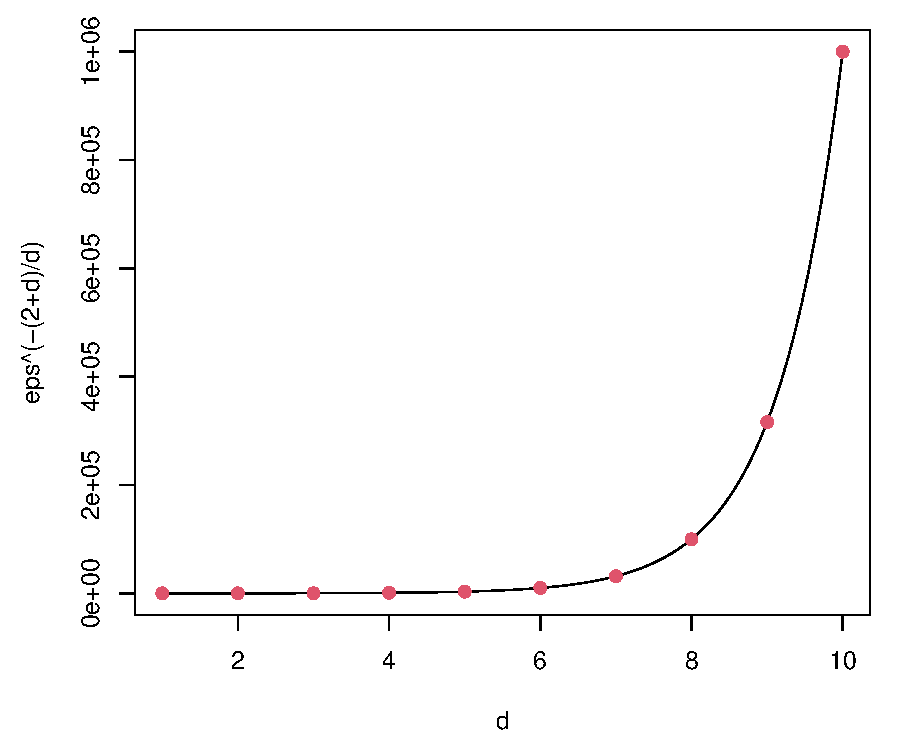
\includegraphics[width=0.6\textwidth]{curse.pdf}
\caption{\it The curse of dimensionality, with $\epsilon=0.1$.} 
\label{fig:curse}
\end{figure}

In fact, this phenomenon is not specific to $k$-nearest neighbors---it is a 
reflection of the \emph{curse of dimensionality}, the principle that estimation
becomes exponentially harder as the number of dimensions increases. 

This is made precise by minimax theory: we cannot hope to do better than the
rate in \eqref{eq:knn_rate} over $C^1(L; [0,1]^d)$, which we write for the space 
of $L$-Lipschitz functions on $[0,1]^d$. It can be shown that
\begin{equation}
\label{eq:lipschitz_lbd}
\inf_{\hf} \, \sup_{f_0 \in C^1(L; [0,1]^d)} \, \E\|\hf - f_0\|_2^2   
\gtrsim n^{-2/(2+d)},
\end{equation}
where the infimum is over all estimators \smash{$\hf$}. This is true for a
uniform input distribution, or for fixed inputs points on a lattice. We will 
revisit (and prove) this in the minimax theory lecture.    

So to circumvent this curse, we'll need to make more assumptions about what it
is that we're looking for in high dimensions. One such example is the additive
model, covered near the end.

\section{Kernel smoothing}

One level up in sophistication is \emph{kernel smoothing} or \emph{kernel 
  regression}. We begin with a kernel function $K : \R \to \R$, satisfying   
\[
\int K(t) \, dt = 1, \quad
\int t K(t) \, dt = 0, \quad
0 < \int t^2 K(t) \, dt < \infty.
\]
Three common examples are the rectangular kernel:
\[
K(t) = 
\begin{cases}
1 & |t| \leq 1 \\
0 & \text{else}
\end{cases},
\]
the Gaussian kernel:
\[
K(t) = \frac{1}{\sqrt{2\pi}} \exp(-t^2/2),
\]
and the Epanechnikov kernel:
\[
K(t) = \begin{cases}
3/4 (1-t^2) & |t| \leq 1 \\ 
0 & \text{else}
\end{cases}.
\]

Given a choice of kernel $K$, and a choice of bandwidth $h>0$, the
(Nadaraya-Watson) kernel regression estimate is then defined as
\begin{equation}
\label{eq:kernel}
\hf(x) = 
\frac{\displaystyle \sum_{i=1}^n K\bigg( \frac{\|x-x_i\|_2}{h} \bigg)  y_i}  
{\displaystyle \sum_{i=1}^n K\bigg( \frac{\|x-x_i\|_2}{h} \bigg)}, 
\end{equation}
Note that kernel smoothing is also a linear smoother \eqref{eq:linear_smoother},
with choice of weights  
\[
w_i(x) = 
\frac{\displaystyle K\bigg ( \frac{\|x-x_i\|_2}{h} \bigg)}
{\displaystyle \sum_{j=1}^n K\bigg ( \frac{\|x-x_j\|_2}{h} \bigg)},
\quad i=1,\dots,n. 
\]

When $K$ is continuous (Gaussian or Epanechnikov), the kernel smoothing
estimator is a continuous moving average of the responses. Compared to the kNN
regression estimator \eqref{eq:knn}, which can be thought of as a raw 
(discontinuous) moving average of nearby responses, the kernel estimator in 
\eqref{eq:kernel} is a smooth moving. See Figure \ref{fig:kernel} for an example.

\begin{figure}[tb]
\centering
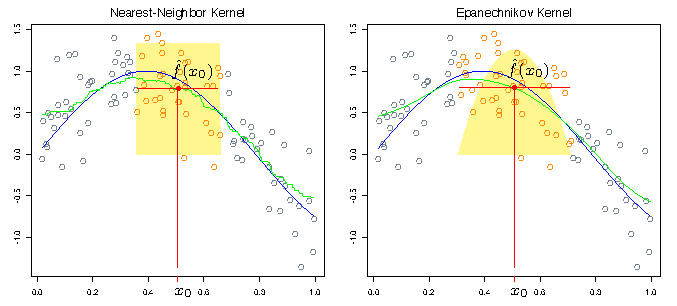
\includegraphics[width=\textwidth]{kernels.pdf}
\caption{\it Comparing kNN and Epanechnikov kernels. Credit: Chapter 6 of
  \citet{hastie2009elements}.}      
\label{fig:kernel}
\end{figure}

Of course, with a rectangular kernel, there is a strong similarity between
kernel smoothing and kNN regression. The difference is that the former performs  
averages over fixed neighborhoods, whereas the latter performs averages over 
adaptive neighborhoods---whose radius at $x$ is defined by the distance to the
$k\th$-nearest neighbor. 

In fact, under suitable conditions, it can be shown that kNN regression acts
like rectangular kernel smoothing with a \emph{density-dependent local
  bandwidth}      
\[
h(x) = \bigg[ \frac{k}{n p(x)} \bigg]^{1/d},
\]
where $p(x)$ is the density of the input distribution at $x$. This is referred
to as the effective kernel for kNN regression. 

\subsection{Local linear regression}

A shortcoming of kernel regression is that it suffers from poor bias at the
boundary of the domain of the input points $x_1,\dots,x_n$. This essentially
happens because of the asymmetry of the kernel weights in such regions. See
Figure \ref{fig:bias} for an illustration. 

\begin{figure}[tb]
\centering
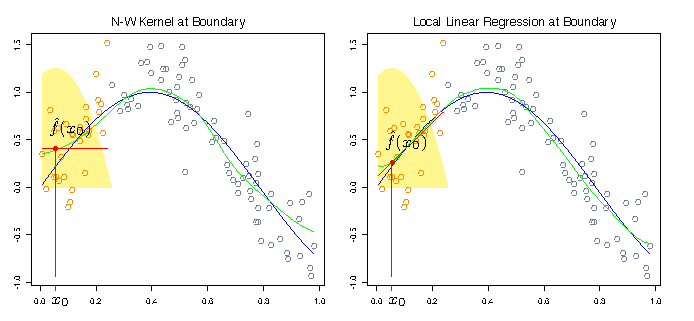
\includegraphics[width=\textwidth]{bias.pdf}
\caption{\it Comparing kernel smoothing to local linear regression; the former
  is biased at the boundary, and the latter is unbiased (to
  first-order). Credit: Chapter 6 of \citet{hastie2009elements}.}  
\label{fig:bias}
\end{figure}

We can alleviate this boundary bias issue by moving from a local constant fit to
a local linear fit. To build intuition, another way to view the kernel smoothing
estimator in \eqref{eq:kernel} is as follows: at each input point $x$, it
employs the estimate \smash{$\hf(x) = \htheta_x$}, which solves 
\[
\minimize_\theta \; \sum_{i=1}^n K\bigg( \frac{\|x-x_i\|_2}{h} \bigg)
(y_i - \theta)^2, 
\]
Instead we could consider forming the local estimate \smash{$\hf(x) = \halpha_x
  + \hbeta_x^\T x$}, where \smash{$\halpha_x,\hbeta_x$} solves
\begin{equation}
\label{eq:llr}
\minimize_{\alpha, \beta} \; \sum_{i=1}^n K\bigg( \frac{\|x-x_i\|_2}{h} \bigg) 
(y_i - \alpha - \beta^\T x_i)^2. 
\end{equation}
This is called \emph{local linear regression}.

We can rewrite the local linear regression prediction \smash{$\hf(x)$} in a more 
evocative way. This is just given by a weighted least squares, so we can write 
\[
\hf(x) = b(x)^\T (B^\T \Omega B)^{-1} B^\T \Omega Y,
\]
where $b(x) = (1,x) \in \R^{d+1}$, $B \in \R^{n \times (d+1)}$ is the matrix
whose $i\th$ row is $b(x_i)$, and $\Omega \in \R^{n \times n}$ is a diagonal 
matrix whose $i\th$ element is $K(\|x-x_i\|_2/h)$. 

Thus we can write the local linear regression prediction more concisely as a
linear smoother \eqref{eq:linear_smoother}: \smash{$\hf(x) = w(x)^\T Y$}, where
the weight vector is
\[
w(x) = \Omega B (B^\T \Omega B)^{-1} b(x).
\]
The vector of fitted values \smash{$\hat{Y} = (\hf(x_1),\dots,\hf(x_n))$} can
be expressed as  
\[
\hat{Y} = 
\left(\begin{array}{c} 
w(x_1)^\T y \\ \vdots \\ w(x_n)^\T y
\end{array}\right)
= B (B^\T \Omega B)^{-1} B^\T \Omega Y,
\]
which should look familiar to you from weighted least squares.

\subsection{Boundary bias calculation}

Now we'll sketch how the local linear fit reduces the bias, fixing (conditioning
on) the training points. Compute at any fixed point $x$,  
\[
\E[\hf(x)] = \sum_{i=1}^n w_i(x) f_0(x_i).
\]
At each $x_i$, using a Taylor expansion of $f_0$ about $x$,
\[
\E[\hf(x)] = f_0(x) \sum_{i=1}^n w_i(x) + \nabla f_0(x)^\T \bigg[
\sum_{i=1}^n (x_i-x) w_i(x) \bigg] + R, 
\]
where the remainder term $R$ contains quadratic and higher-order terms, and
under regularity conditions, is small. One can check (via direct algebra) that
\[
\sum_{i=1}^n w_i(x) = 1 \quad \text{for both kernel smoothing and local linear
  regression}. 
\]
On the other hand 
\begin{align*}
\sum_{i=1}^n (x_i-x) w_i(x) &\not= 0 
\quad \text{for kernel smoothing, and} \\
\sum_{i=1}^n (x_i-x) w_i(x) &= 0 
\quad \text{for local linear regression}. 
\end{align*}
Indeed the first-order bias term \smash{$\nabla f_0(x)^\T (\sum_{i=1}^n (x_i-x) 
  w_i(x))$} will be generally large for kernel smoothing for $x$ near the
boundary. Meanwhile, for local linear regression, \smash{$\E[\hf(x)] = f_0(x) +
  R$}, which means that it is unbiased to first-order (at any $x$, including $x$
near the boundary).    

\subsection{Universal consistency}

Like kNN regression, the kernel smoothing estimator is universally consistent,
meaning that under essentially no assumptions we can still get
\smash{$\E\|\hf-f_0\|_2^2 \to 0$} as $n \to \infty$, provided we use a
nonnegative compactly supported kernel $K$ and bandwidth $h=h_n$ satisfying 
$h_n \to 0$ and $nh_n^d \to \infty$ as $n \to \infty$. See Chapter 5.2 of
\citet{gyorfi2002distribution}. 

Unfortunately, local linear regression does not share this property, and fails
to be universally consistent. In theory, this can be rectified using a suitable
truncation trick (restricting the domain in the weighted least squares problem
\eqref{eq:llr} that defines each local linear regression estimate to be an
$\ell_\infty$ ball whose radius diverges with $n$). See Chapter 5.3 of 
\citet{gyorfi2002distribution}. However, we should note that this truncated
estimator doesn't seem to be in common use in practice.  

\subsection{Rate of convergence}

Assuming that $f_0 \in C^1(L; [0,1]^d)$, the underlying regression function
$f_0$ is Lipschitz continuous on $[0,1]^d$ for some constant $L>0$, and we place
mild conditions on the input distribution, the kernel smoothing estimator with a  
rectangular kernel and bandwidth \smash{$h \asymp n^{-1/(2+d)}$} satisfies    
\begin{equation}
\label{eq:kernel_rate}
\E\|\hf - f_0\|_2^2 \lesssim n^{-2/(2+d)} \quad \text{in probability},
\end{equation}
just like kNN regression. Similar results hold for more general nonnegative
compactly supported kernels.

Proof sketch: as usual, denote $\sigma^2 = \Var(\epsilon_0)$, fix the input
points (condition on them), and condition on $x_0$. We'll compute the bias and
variance separately. In fact we already did the bias calculation, using a
first-order Taylor expansion of $f_0$: 
\[
\E[\hf(x_0)] = f_0(x_0) + \nabla f_0(x_0)^\T \bigg[\sum_{i=1}^n (x_i-x_0)
w_i(x_0) \bigg] + R,  
\]
where $R$ is a small remainder term that we'll ignore. The Lipschitz condition
implies that $f_0$ is almost everywhere differentiable with $\|\nabla
f_0\|_\infty \leq L$ (by Rademacher's theorem). Hence for the squared bias,
\[
\Bias^2(\hf(x_0) | x_0) 
\leq L^2 \bigg\| \sum_{i=1}^n (x_i-x_0) w_i(x_0) \bigg\|_2^2 
\leq L^2 \bigg[ \sum_{i=1}^n \|x_i-x_0\|_2 w_i(x_0) \bigg]^2.
\]
Now we use the fact that that $K(t) = 0$ for $|t| > 1$. Then we can further
bound the sum above: 
\[
\Bias^2(\hf(x_0) | x_0) 
\leq L^2 h^2 \bigg[ \sum_{i=1}^n w_i(x_0) \bigg]_2^2
= L^2 h^2.
\]
Now for the variance, using the fact that $y_i$, $i=1,\dots,n$ are independent
with variance $\sigma^2>0$,
\[
\Var(\hf(x_0) | x_0) 
= \sigma^2 \sum_{i=1}^n w_i(x_0)^2 
\leq \sigma^2 \bigg[ \max_{i=1,\dots,n} w_i(x_0) \bigg] 
\bigg[ \sum_{i=1}^n w_i(x_0) \bigg]  
\leq \sigma^2 \bigg[ \max_{i=1,\dots,n} w_i(x_0) \bigg].
\]
For the rectangular kernel, using $P_n$ for the empirical distribution of
$x_1,\dots,x_n$, we have 
\[
w_i(x_0) = \frac{1\{ \|x_0-x_i\|_2 \leq h \}}{n P_n(B(x_0, h)) } \leq
\frac{1}{cnh^d},
\]
where $B(x_0,h)$ is the $\ell_2$ ball centered at $x_0$ with radius $h$, and we
used the fact that it can be shown that with high probability (over the
distribution of $x_1,\dots,x_n$) that $P_n(S) \geq c \cdot \mathrm{vol}(S)$ for
any set $S$ that is not too small, where $c>0$ is a constant. Our bias-variance
upper bound on the risk is hence:
\[
L^2 h^2 + \frac{\sigma^2}{cnh^d}.
\]
Balancing the two terms so that they are equal gives \smash{$h^{2+d} \asymp
  n^{-1}$}, i.e., \smash{$h \asymp n^{-1/(2+d)}$}. And plugging this in gives
the error rate of \smash{$n^{-2/(2+d)}$}, as claimed.   

\subsection{Higher-order smoothness}

To define and study higher-order smoothness classes, we'll need some more
notation: given a multi-index $\alpha=(\alpha_1,\dots,\alpha_d) \in \Z^d_+$, we
write  $|\alpha| = \alpha_1 + \cdots \alpha_d$ and 
\[
D^\alpha f = \frac{\partial^{|\alpha|} f}{\partial x_1^{\alpha_1} \partial
  x_2^{\alpha_2} \dots \partial x_d^{\alpha_d}}.
\]
For an integer $r \geq 0$, exponent $0 < \gamma \leq 1$, radius $L>0$, and
domain $\Omega$, we can now define the H{\"o}lder class
\[
C^{r+\gamma}(L; \Omega) = \Big\{ f : \Omega \to \R \,:\, | D^\alpha f (x) -
D^\alpha f(y) | \leq L \|x-y\|_2^\gamma \; \text{for all $|\alpha| = r$, and
  $x,y \in \Omega$} \Big\}. 
\]
Note that $C^1(L; \Omega)$ is simply the space of all $L$-Lipschitz functions on
$\Omega$. Likewise, for an integer $k \geq 1$, $C^k(L; \Omega)$ is the space of
all functions on $\Omega$ whose order $k-1$ partial derivatives are all
$L$-Lipschitz. 

It can be shown that a minimax lower bound over $C^s(L; [0,1]^d)$, for a
constant $L>0$, is    
\begin{equation}
\label{eq:holder_lbd}
\inf_{\hf} \, \sup_{f_0 \in C^s(L; [0,1]^d)} \, \E\|\hf - f_0\|_2^2   
\gtrsim n^{-2s/(2s+d)},
\end{equation}
which generalizes the result we cited earlier for Lipschitz functions in
\eqref{eq:lipschitz_lbd}. Again, we'll study this in detail in the minimax
theory lecture. 

So now let's think about rate optimal estimators. We saw from
\eqref{eq:knn_rate} and \eqref{eq:kernel_rate} that both kNN regression and
kernel smoothing are minimax rate optimal over $C^1(L; [0,1]^d)$. But what about
$C^s(L; [0,1]^d)$, for $s>1$? Can these estimators ``track'' the smoothness of
$f_0$? 

The answer is kind of both ``yes'' and ``no''. For the ``yes'' part, it turns
out that kernel smoothing can still achieve the optimal convergence rate over   
$C^{1.5}(L; [0,1]^d)$, and the same is conjectured to be true of kNN. See
Chapters 5.3 and 6.3 of \citet{gyorfi2002distribution}.

For the ``no'' part: neither achieves the optimal rate over $C^2(L;
[0,1]^d)$. See again Chapters 5.3 and 6.3 of \citet{gyorfi2002distribution}. An
important remark: here we see a big discrepancy between a pointwise analysis and
$L^2$ theory. It can be shown that both kernel smoothing and kNN regression
satisfy   
\[
\E\big[ (\hf(x_0) - f_0(x_0))^2 \big] \lesssim n^{-4/(4+d)} \quad \text{for any
  fixed $x_0 \in (0,1)^d$}.   
\]
when $f_0 \in C^2(L; [0,1]^d)$. But the same is not true when we integrate over
$x_0$, because the boundary bias inflates the error rate, for both methods.  

Lastly, if you recall, we already talked about how to fix boundary bias ... 
local linear regression to the rescue! As one would hope, this is indeed rate
optimal over $C^2(L; [0,1]^d)$, i.e., assuming that $f_0 \in C^2(L; [0,1]^d)$,
and we place mild conditions on the input distribution as usual, the local
linear regression estimator with bandwidth \smash{$h \asymp n^{-1/(4+d)}$} 
satisfies      
\begin{equation}
\label{eq:kernel_rate}
\E\|\hf - f_0\|_2^2 \lesssim n^{-4/(4+d)} \quad \text{in probability},
\end{equation}
for general nonnegative compactly supported kernels. We can see this matches the
rate in \eqref{eq:holder_lbd} for $s=2$.

\subsection{Local polynomials and higher-order kernels}

How can we get optimal error rates for even smoother functions, in $C^s(L;
[0,1]^d)$ for $s > 2$? With kernels there are basically two options: use
local polynomials, or use higher-order kernels.

Local polynomials build on the idea behind local linear regression (as an
extension of kernel smoothing). Consider $d=1$, for concreteness. Define
\smash{$\hf(x) = \halpha_x + \sum_{j=1}^k \hbeta_{x,j} x^j$}, where the
parameters \smash{$\halpha_x,\hbeta_{x,1},\dots,\hbeta_{x,k}$} now solve 
(cf.\ problem \eqref{eq:llr}):
\begin{equation}
\label{eq:local_poly}
\minimize_{\alpha, \beta_1,\dots,\beta_k} \; \sum_{i=1}^n K\bigg(
\frac{\|x-x_i\|_2}{h} \bigg) \bigg(y_i - \alpha - \sum_{j=1}^k \beta_j x_i^j 
\bigg)^2. 
\end{equation}
This is called ($k\th$ order) \emph{local polynomial regression}. As before, we 
can express the prediction at $x$ as
\[
\hf(x) = b(x)(B^\T \Omega B)^{-1} B^\T \Omega Y = w(x)^\T Y,
\]
where now $b(x) = (1,x,\dots,x^k)$, $B$ is an $n \times (k+1)$, $B \in \R^{n 
  \times (k+1)}$ is the matrix whose $i\th$ row is $b(x_i)$, and $\Omega \in
\R^{n \times n}$ is the same diagonal matrix with kernel weights as
before. Hence again, local polynomial regression is a linear smoother. 

In multiple dimensions, $d>1$, local polynomials become kind of tricky to fit,
because of the explosion in terms of the number of parameters we need to
represent a $k\th$ order polynomial in $d$ variables. Hence, an interesting
alternative is to return back kernel smoothing but use a \emph{higher-order 
  kernel}. A kernel function $K$ is said to be of order $k$ provided that
\[ 
\int K(t) \, dt = 1, \quad
\int t K(t) \, dt = 0, \; j=1,\dots,k-1, \quad
0 < \int t^k K(t) \, dt < \infty.
\]
This means that the kernels we were looking at so far were of order 2. An
example of a 4th order kernel is 
\[
K(t) = \frac{3}{8}(3-5t^2) 1\{|t|\leq 1\}, 
\]
plotted in Figure \ref{fig:order4}. Notice that it takes negative values! 
(Higher-order kernels, in fact, have an interesting connection to smoothing
splines, which we'll learn a bit later on.)

\begin{figure}[tb]
\centering
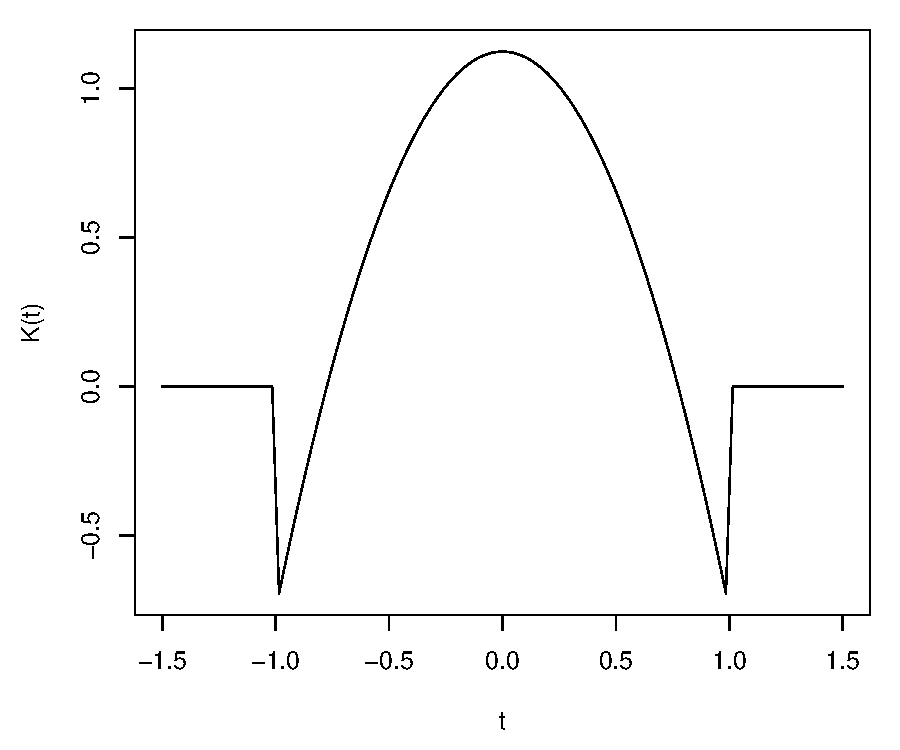
\includegraphics[width=0.6\textwidth]{order4.pdf}
\caption{\it A higher-order kernel function---specifically, a kernel of  order 
  4.}   
\label{fig:order4}
\end{figure}

Both local polynomials and higher-order kernels can achieve optimal rates over
higher-order H{\"older} classes, where the order of the polynomial or kernel is
adjusted with the order of smoothness. We do not give the details here (but see, 
e.g., Chapter 1.6.1 of \citet{tsybakov2009introduction} for an analysis of local 
polynomials). 

\bibliographystyle{plainnat}
\bibliography{../../common/ryantibs.bib}

\end{document}
